\documentclass[a4paper,11pt]{article}

%%%%%%%% CREATE DOCUMENT STRUCTURE %%%%%%%%
%% Language and font encodings
\usepackage[italian]{babel}
\usepackage[utf8x]{inputenc}
\usepackage[T1]{fontenc}

%% Sets page size and margins
\usepackage[a4paper,top=3cm,bottom=2cm,left=2cm,right=2cm,marginparwidth=1.75cm]{geometry}

%% Useful packages
\usepackage{amsmath}
\usepackage{amssymb}
\usepackage{amsfonts} % for /mathbb and similar math symbols
\usepackage{graphicx}
\usepackage[colorlinks=true, allcolors=blue]{hyperref}
\usepackage{caption}
\usepackage{subcaption}
\usepackage{float}
\usepackage{titling}
\usepackage{blindtext}
\usepackage[square,sort,comma,numbers]{natbib}
\usepackage{xcolor}

\newcommand{\HRule}{\rule{\linewidth}{0.5mm}} 	% horizontal line and its thickness


%%%%%%%% DOCUMENT %%%%%%%%
\begin{document}

%%%% Title Page
\begin{titlepage}
\center
% Some logo, optional

\includegraphics[width=0.6\textwidth]{img/unipi-logo.png}\\[1cm]

% University
\textsc{\LARGE Università di Pisa, Dipartimento di Informatica}\\[1cm]

% Document info
\textsc{\Large Laboratorio di Basi di dati - A.A. 2021-2022}\\[0.2cm]
\textsc{\large Docente: Giovanna Rosone}\\[1cm]

% Assignment title (enclosed between horizontal lines
\HRule \\[0.8cm]
{ \huge \bfseries Specifica delle operazioni}\\[0.7cm]
\HRule \\[2cm]

% Author and date
\Huge \emph{Gruppo 2}\\[0.5cm]
\large Francesco Nicolò\\Roberto Puggioni\\Jacopo Raffi\\Nicola Vetrini\\[1.5cm]
{\large \today}\\[5cm]

\vfill
\end{titlepage}

\clearpage
\tableofcontents
\clearpage

\section{Introduzione}
Il compito di questo gruppo è stata l'implementazione delle operazioni relative alle classi Autori, Opere e Descrizioni dello schema concettuale. Il lavoro è stato diviso internamente in due sottogruppi: Jacopo Raffi e Francesco Nicolò si sono occupati delle operazioni relative alle Opere, mentre Roberto Puggioni e Nicola Vetrini di quelle relative ad Autori e Descrizioni. La verifica e l'estensione delle funzionalità sono state svolte da tutti i membri su tutte le operazioni, durante la scrittura e il debug si è seguita l'idea secondo cui il primo componente che si accorgesse di dover effettuare modifiche lo facesse al momento o avvisasse la coppia di colleghi a seconda della situazione.\\
Nel pacchetto realizzato vi sono due pagine principali: il menuAutori ed il menuOpere, dai
quali è possibile scegliere l'operazione da eseguire. Alcuni collegamenti sono visibili soltanto se si hanno determinate autorizzazioni, secondo la specifica indicata nella tabella \textit{Diritti ed Operazioni} fornita dal gruppo di progettazione logica.\\
Dato che l'implementazione ha portato a realizzare le operazioni come una serie di procedure correlate, nel documento è riportato in ogni operazione l'elenco delle procedure
coinvolte, comprese quelle che non corrispondono a delle pagine visibili all'utente

% Ogni capitolo incluso di seguito include la specifica delle operazioni relative all
% corrispondente classe dello schema logico
%%%%%%%%%%%%%%%%%%%%%%%%%%%
%     Visualizza Opera    %
%%%%%%%%%%%%%%%%%%%%%%%%%%%
\subsection{Visualizzazione}
\begin{itemize}
	\item \textbf{Procedure coinvolte}: VisualizzaOpera
	\item \textbf{Obiettivo}: Visualizzare i dettagli e le descrizioni di un'Opera nella base di dati
	\item \textbf{Parametri}:
	\begin{enumerate}
		\item \textbf{operaID}: in NUMBER
		\item \textbf{lingue}: in VARCHAR2, la lingua delle decrizioni da visualizzare
		\item \textbf{livelli}: in VARCHAR2, il livello delle descrizioni da visualizzare
	\end{enumerate}
	\item \textbf{Risultato}: Visualizza l'Opera richiesta e le descrizioni presenti
	\item \textbf{Usa}: Opere, AutoriOpere, Descrizioni, SaleOpere, Stanze, Sale, Musei, Autori
	\item \textbf{Modifica}: nessuna
	\item \textbf{Precondizioni}:
	\begin{itemize}
		\item $\exists! opera \in Opere : opera.IdOpera = operaID$
	\end{itemize}
	\item \textbf{Postcondizioni}: nessuna
\end{itemize}

%%%%%%%%%%%%%%%%%%%%%%%%%%%
%     Inserisci Opera     %
%%%%%%%%%%%%%%%%%%%%%%%%%%%
\subsection{Inserimento}
\begin{itemize}
	\item \textbf{Procedure coinvolte}: InserisciOpera, ConfermaDatiOpera, InserisciDatiOpera
	\item \textbf{Obiettivo}: Inserisce una nuova Opera nel database
	\item \textbf{Parametri}:
	\begin{enumerate}
		\item \textbf{Titolo}: in VARCHAR2
		\item \textbf{Anno}: in VARCHAR2
		\item \textbf{FinePeriodo}: in VARCHAR2, \textbf{opzionale}, fine del periodo di realizzazione 
		\item \textbf{IdMusei}: in NUMBER
	\end{enumerate}
	\item \textbf{Risultato}: Inserisce l'Opera richiesta nella base di dati, oppure restituisce un errore
	\item \textbf{Errori}: 
	\begin{itemize}
	%\item L'Opera con i dati inseriti è già presente nel database
		\item Parametri obbligatori con valore nullo (solo se chiamata a ConfermaDatiOpera senza passare da InserisciOpera)
		\item Parametri newAnno e newFineperiodo presentano caratteri non numerici
	\end{itemize}
	\item \textbf{Usa}: Opere, Musei, AppartieneA
	\item \textbf{Modifica}: Opere
	\item \textbf{Precondizioni}:
	\begin{itemize}
		\item $MuseoID \ne null \land Titolo \ne null \land Anno \ne null$
		\item $\exists x \in Musei : x.IdMuseo = MuseoID$
		%\item $\nexists x \in Opere : x.Museo = MuseoID \land x.Titolo = Titolo \land x.Anno = Anno$
		\item $|Opere| = n$
	\end{itemize}
	\item \textbf{Postcondizioni}:
	\begin{itemize}
		\item $\exists! opera \in Opere : opera = (IdOpera.nextval, titolo, anno, fineperiodo, museo, 1, 0)$
	\end{itemize}
\end{itemize}

%%%%%%%%%%%%%%%%%%%%%%%%%%%
%     Modifica Opera      %
%%%%%%%%%%%%%%%%%%%%%%%%%%%
\subsection{Modifica}
\begin{itemize}
	\item \textbf{Procedure coinvolte}: ModificaOpera, ConfermaUpdateOpera, UpdateOpera
	\item \textbf{Obiettivo}: Modifica un'Opera presente nel database
	\item \textbf{Parametri}:
	\begin{enumerate}
		\item \textbf{OperaID}: in NUMBER
		\item \textbf{newTitolo}: in VARCHAR2
		\item \textbf{newAnno}: in VARCHAR2
		\item \textbf{newFineperiodo}: in VARCHAR2, opzionale
		\item \textbf{newIdMusei}: in NUMBER
	\end{enumerate}
	\item \textbf{Risultato}: Modifica l'Opera specificata se esiste nella base di dati, errore altrimenti (la base di dati rimane inalterata)
	\item \textbf{Errori}: 
	\begin{itemize}
		\item L'Opera con OperaID non è presente nel database
		\item Parametri obbligatori con valore nullo
		\item Parametri newAnno e newFineperiodo presentano caratteri non numerici
	\end{itemize}
	\item \textbf{Usa}: Opere, Musei
	\item \textbf{Modifica}: Opere
	\item \textbf{Precondizioni}:
	\begin{itemize}
		\item $\exists x \in Opere : x.IdOpera = OperaID$
		\item $newTitolo \ne null \land newAnno \ne null \land newFineperiodo \ne null \land newIdMusei \ne null$
		\item $\exists x \in Musei : x.IdMuseo = newmuseum$
		\item $|Opere| = n$
	\end{itemize}
	\item \textbf{Postcondizioni}: se $x \in Opere \land x.IdOpera = OperaID$
	\begin{itemize}
		\item $x.Titolo := newtitle$
		\item $x.Anno := newyear$
		\item $x.Fineperiodo := newFinePeriodo$
		\item $x.Museo := newIdMusei$
		\item $|Opere| = n$
	\end{itemize}
	\item \textbf{Note}:
	%% TODO: add link aggiungiAutore/rimuoviAutore
	Nel form di modifica è possibile anche aggiungere o rimuovere autori, se autorizzati.
	Per realizzare tale operazione viene richiamata la procedura \hyperref[AggiuntaAutore]{\textbf{Aggiunta autore}}
	o \hyperref[RimozioneAutoreOpera]{\textbf{Rimozione autore}} e poi si è rediretti al
	menu delle opere al termine dell'operazione
\end{itemize}

%%%%%%%%%%%%%%%%%%%%%%%%%%%
%     Elimina Opera       %
%%%%%%%%%%%%%%%%%%%%%%%%%%%
\subsection{Eliminazione}
\begin{itemize}
	\item \textbf{Procedure coinvolte}: EliminazioneOpera, RimozioneOpera
	\item \textbf{Obiettivo}: Elimina un'opera dalla lista di quelle visibili agli Utenti, senza rimuoverla dal database
	\item \textbf{Parametri}:
	\begin{enumerate}
		\item \textbf{OperaID}: in NUMBER
	\end{enumerate}
	\item \textbf{Risultato}: L'opera individuata da operaID viene resa non visibile agli utenti, ma se e solo se non è al momento esposta in alcun museo. Se lo è l'eliminazione non è concessa e la base di dati non è alterata
	\item \textbf{Errori}: 
	\begin{itemize}
		\item L'Opera individuata da operaID è in esposizione in un museo
		\item L'Opera con OperaID non è presente nel database
	\end{itemize}
	\item \textbf{Usa}: Opere, SaleOpere, AutoriOpere, Descrizioni
	\item \textbf{Modifica}: Opere
	\item \textbf{Precondizioni}:
	\begin{itemize}
		\item $\exists x \in Opere : x.IdOpera = OperaID$
		\item $\nexists x \in SaleOpere : x.Opera=operaID \land x.DataUscita = null$
	\end{itemize}
	\item \textbf{Postcondizioni}:
	\begin{itemize}
		\item $\exists x \in Opere : x.IdOpera = operaID \land x.Eliminato = 1$
	\end{itemize}
	%% TODO: controllare semantica
	\item \textbf{Note}: Le informazioni correlate all'opera non sono alterate
\end{itemize}

%%%%%%%%%%%%%%%%%%%%%%%%%%%
%     Rimuovi Opera       %
%%%%%%%%%%%%%%%%%%%%%%%%%%%
\subsection{Rimozione}
\begin{itemize}
	\item \textbf{Procedure coinvolte}: EliminazioneDefinitivaOpera, RimozioneDefinitivaOpera
	\item \textbf{Obiettivo}: Rimuove un'Opera dal database
	\item \textbf{Parametri}:
	\begin{enumerate}
		\item \textbf{OperaID}: in NUMBER
	\end{enumerate}
	\item \textbf{Risultato}: L'opera individuata da operaID viene rimossa dalla base di dati
	\item \textbf{Errori}: 
	\begin{itemize}
		\item L'Opera individuata da operaID è in esposizione in un museo
		\item L'Opera con OperaID non è presente nel database
	\end{itemize}
	\item \textbf{Usa}: Opere, SaleOpere, AutoriOpere, Descrizioni
	\item \textbf{Modifica}: Opere, SaleOpere, AutoriOpere, Descrizioni
	\item \textbf{Precondizioni}:
	\begin{itemize}
		\item $\exists x \in Opere : x.IdOpera = OperaID$
		\item $\nexists x \in SaleOpere : x.Opera=operaID \land x.DataUscita = null$
	\end{itemize}
	\item \textbf{Postcondizioni}:
	\begin{itemize}
		\item $\nexists x \in Opere : x.IdOpera = operaID$
	\end{itemize}
	%% TODO: controllare semantica
	\item \textbf{Note}: Tutte le tracce dell'opera dalle tabelle modificate sono rimosse
\end{itemize}

%%%%%%%%%%%%%%%%%%%%%%%%%%%
%  Aggiunta Autore Opera  %
%%%%%%%%%%%%%%%%%%%%%%%%%%%
% Si intende l'aggiunta di un autore già esistente nella base di dati
\label{AggiuntaAutore}
\begin{itemize}
	\item \textbf{Procedure coinvolte}: AggiungiAutore
	\item \textbf{Obiettivo}: Aggiunge un Autore ad un'Opera, se entrambe le entità sono presenti nella base di dati
	\item \textbf{Parametri}:
	\begin{enumerate}
		\item \textbf{OperaID}: in NUMBER
		\item \textbf{AutoreID}: in NUMBER
		\item \textbf{lingue}: in VARCHAR2, opzionale, per redirect alla visualizzazione
	\end{enumerate}
	\item \textbf{Risultato}: Aggiunge l'autore con l'ID indicato all'Opera individuata dall'ID dato.\\
	Se l'autore specificato compare già tra gli autori dell'Opera, allora la base di dati rimane inalterata
	\item \textbf{Errori}: 
	\begin{itemize}
		\item L'autore individuato da AuthorID è già stato aggiunto come autore di quest'Opera
	\end{itemize}
	\item \textbf{Usa}: Autori, AutoriOpere
	\item \textbf{Modifica}: AutoriOpere
	\item \textbf{Precondizioni}:
	\begin{itemize}
		\item $\exists x \in Opere : x.IdOpera = OperaID$
		\item $\exists y \in Autori : y.IdAutore = AuthorID$
		\item $\nexists z \in AutoriOpere : z.IdAutore = AuthorID \land z.IdOpera = OperaID$
		\item $|AutoriOpere| = n$
	\end{itemize}
	\item \textbf{Postcondizioni}:
	\begin{itemize}
		\item $\exists z \in AutoriOpere : z.IdAutore = AuthorID \land z.IdOpera = OperaID$
		\item $|AutoriOpere| = n + 1$
	\end{itemize}
\end{itemize}

\label{RimozioneAutoreOpera}
\subsection{Rimozione Autore Opera}
\begin{itemize}
	\item \textbf{Procedure coinvolte}: RimozioneAutoreOpera, RimuoviAutoreOpera
	\item \textbf{Obiettivo}: Rimuove un Autore da un'Opera, se entrambe le entità sono presenti nella base di dati ed è presente l'associazione tra autore ed opera
	\item \textbf{Parametri}:
	\begin{enumerate}
		\item \textbf{OperaID}: in NUMBER
		\item \textbf{AutoreID}: in NUMBER
		\item \textbf{lingue}: in VARCHAR2, opzionale, per redirezione verso visualizzazione opera
	\end{enumerate}
	\item \textbf{Risultato}: Rimuove l'autore con l'ID indicato dall'Opera individuata dall'ID dato.\\
	Se l'autore specificato non compare già tra gli autori dell'Opera, allora la base di dati rimane inalterata
	\item \textbf{Errori}:
	\begin{itemize}
		\item L'autore individuato da AuthorID non è associato all'opera individuata da OperaID
	\end{itemize}
	\item \textbf{Usa}: Autori, AutoriOpere
	\item \textbf{Modifica}: AutoriOpere
	\item \textbf{Precondizioni}:
	\begin{itemize}
		\item $\exists x \in Opere : x.IdOpera = OperaID$
		\item $\exists y \in Autori : y.IdAutore = AuthorID$
		\item $\exists z \in AutoriOpere : z.IdAutore = AuthorID \land z.IdOpera = OperaID$
		\item $|AutoriOpere| = n$
	\end{itemize}
	\item \textbf{Postcondizioni}:
	\begin{itemize}
		\item $\nexists z \in AutoriOpere : z.IdAutore = AuthorID \land z.IdOpera = OperaID$
		\item $|AutoriOpere| = n - 1$
	\end{itemize}
\end{itemize}

\subsection{Statistiche e monitoraggio}

\subsubsection{Storico prestiti dell’Opera}
\begin{itemize}
    \item \textbf{Procedure Coinvolte}: SpostamentiOpera
    \item \textbf{Obiettivo}: Mostrare lo storico dei prestiti di una determinata opera
    \item \textbf{Parametri}:
	\begin{enumerate}
		\item \textbf{OperaID}: in NUMBER
	\end{enumerate}
	\item \textbf{Risultato}: Mostra il proprietario, il destinatario e il periodo del prestito
	\item \textbf{Usa}: Musei, SaleOpere, Opere, Stanze
	\item \textbf{Modifica}: niente
	\item \textbf{Precondizioni}:
	\begin{itemize}
		\item \exists x \in Opere : x.IdOpera = OperaID\\
		\item \exists y \in SaleOpera : y.opera = operaID
		\item \exists z \in SaleOpere : \exists w \in Stanze : z.idStanza = w.sala \land w.Opera = OperaID\\
	\end{itemize}
	\item \textbf{Postcondizioni}: nessuna
\end{itemize}
\subsubsection{Autori dell’Opera}
\subsubsection{Tipo Sala in cui si trova l’Opera}
\subsubsection{Descrizioni dell’Opera}

\subsubsection{Lista Opere ordinate per numero di Autori in ordine decrescente}
\begin{itemize}
	\item \textbf{Procedure coinvolte}: statisticheOpere
	\item \textbf{Obiettivo}: Mostra le opere con il maggior numero di autori
	\item \textbf{Parametri}:
	\begin{enumerate}
		\item \textbf{museoID}: in NUMBER
	\end{enumerate}
	\item \textbf{Risultato}: Mostra il nome delle prime tre opere, se museoID $\neq 0$ relative a quel museo altrimenti tra tutti i musei, con il maggior numero di autori e il numero di autori dell'opera
	\item \textbf{Errori}: nessuno
	\item \textbf{Usa}: Opere, AutoriOpere, Musei
	\item \textbf{Modifica}: niente
	\item \textbf{Precondizioni}:
	\begin{itemize}
		\item |opere| \ge 3
	\end{itemize}
	\item \textbf{Postcondizioni}: nessuna
\end{itemize}

\subsubsection{Opere non spostata da più tempo (le tre più vecchie)}
\begin{itemize}
	\item \textbf{Procedure coinvolte}: statisticheOpere
	\item \textbf{Obiettivo}: Mostra le opere non spostate da più tempo
	\item \textbf{Parametri}:
	\begin{enumerate}
		\item \textbf{museoID}: in NUMBER
	\end{enumerate}
	\item \textbf{Risultato}: Mostra il nome delle prime tre opere, se museoID $\neq 0$ relative a quel museo altrimenti tra tutti i musei, non spostate da più tempo e per quanti giorni non sono state spostate
	\item \textbf{Errori}: nessuno
	\item \textbf{Usa}: Opere, saleOpere, Musei
	\item \textbf{Modifica}: niente
	\item \textbf{Precondizioni}:
	\begin{itemize}
		\item |opere| \ge 3
	\end{itemize}
	\item \textbf{Postcondizioni}: nessuna
\end{itemize}

\subsubsection{Opere esposte per più tempo (le tre più vecchie)}
\begin{itemize}
	\item \textbf{Procedure coinvolte}: statisticheOpere
	\item \textbf{Obiettivo}: Mostra le opere esposte per più tempo
	\item \textbf{Parametri}:
	\begin{enumerate}
		\item \textbf{museoID}: in NUMBER
	\end{enumerate}
	\item \textbf{Risultato}: Mostra il nome delle prime tre opere, se museoID $\neq 0$ relative a quel museo altrimenti tra tutti i musei, esposte da più tempo e per quanti giorni sono state esposte
	\item \textbf{Errori}: nessuno
	\item \textbf{Usa}: Opere, saleOpere, Musei
	\item \textbf{Modifica}: niente
	\item \textbf{Precondizioni}:
	\begin{itemize}
		\item $|opere| \ge 3$ 
	\end{itemize}
	\item \textbf{Postcondizioni}: nessuna
\end{itemize}
\subsubsection{Età media delle opere}

\subsubsection{Ordinamento per anno di realizzazione (le tre più vecchie)}
\begin{itemize}
	\item \textbf{Procedure coinvolte}: statisticheOpere
	\item \textbf{Obiettivo}: Mostra le opere più antiche
	\item \textbf{Parametri}:
	\begin{enumerate}
		\item \textbf{museoID}: in NUMBER
	\end{enumerate}
	\item \textbf{Risultato}: Mostra il nome delle prime tre opere, se museoID $\neq 0$ relative a quel museo altrimenti tra tutti i musei, più antiche e l'età, in anni, dell'opera
	\item \textbf{Errori}: nessuno
	\item \textbf{Usa}: Opere, Musei
	\item \textbf{Modifica}: niente
	\item \textbf{Precondizioni}:
	\begin{itemize}
		\item |opere| \ge 3
	\end{itemize}
	\item \textbf{Postcondizioni}: nessuna
\end{itemize}

\clearpage

%%%%%%%%%%%%%%%%%%%%%%%%%%%%%%%
%   Operazioni sugli Autori   %
%%%%%%%%%%%%%%%%%%%%%%%%%%%%%%%
\section{Operazioni sugli Autori}

%%%%%%%%%%%%%%%%%%%%%%%%%%%%%%
%     Visualizza Autore      %
%%%%%%%%%%%%%%%%%%%%%%%%%%%%%%
\subsection{Visualizzazione}
\begin{itemize}
	\item \textbf{Operazione}: ModificaAutore (con parametro operazione = 0)
	\item \textbf{Obiettivo}: Visualizza le informazioni relative ad un Autore presente nel database
	\item \textbf{Parametri}:
	\begin{enumerate}
		\item \textbf{authorID}: in number
		\item \textbf{operazione}: in number
		\item \textbf{caller}: in varchar2 (nome della procedura chiamante, per redirect)
		\item \textbf{callerParams}: in varchar2 (parametri del chiamante)
	\end{enumerate}
	\item \textbf{Risultato}: Visualizza i dati relativi all'autore identificato da AuthorID, se presente nel database, restituisce un errore altrimenti
	\item \textbf{Errori}: 
	\begin{itemize}
		\item L'Autore identificato da AuthorID non è presente nel database
	\end{itemize}
	\item \textbf{Usa}: Autori
	\item \textbf{Modifica}: nessuno
	\item \textbf{Precondizioni}:
	\begin{itemize}
		\item $\exists x \in Autori : x.IdAutore = AuthorID$
	\end{itemize}
	\item \textbf{Postcondizioni}: nessuna
	\item \textbf{Note}: Oltre ai dettagli dell'autore è presente un form che permette di 
	visualizzare alcune statistiche relative all'autore:  \hyperref[OpereRealizzate]{\textbf{Opere realizzate}}, 
	\hyperref[MuseiOpereEsposte]{\textbf{Musei con opere esposte}},
	\hyperref[Collaborazioni]{\textbf{Collaborazioni effettuate}}.
\end{itemize}

%%%%%%%%%%%%%%%%%%%%%%%%%%%%%%
%      Inserisci Autore      %
%%%%%%%%%%%%%%%%%%%%%%%%%%%%%%
\subsection{Inserimento}
\begin{itemize}
	\item \textbf{Procedure coinvolte}: InserisciAutore, ConfermaDatiAutore, InserisciDatiAutore
	\item \textbf{Obiettivo}: Inserisce un nuovo autore nel database
	\item \textbf{Parametri}:
	\begin{enumerate}
		\item \textbf{authName}: in varchar2
		\item \textbf{authSurname}: in varchar2
		\item \textbf{dataNascita}: in date
		\item \textbf{dataMorte}: in date
		\item \textbf{nation}: in varchar2
	\end{enumerate}
	\item \textbf{Risultato}: Inserisce un nuovo autore nella tabella Autori con i dati specificati dai parametri, se consentito
	\item \textbf{Errori}: 
	\begin{itemize}
		\item È già presente nel database un autore con gli stessi dati
		\item La data di nascita dell'autore è posteriore alla data di morte
	\end{itemize}
	\item \textbf{Usa}: Autori
	\item \textbf{Modifica}: Autori
	\item \textbf{Precondizioni}:
	\begin{itemize}
		\item $authName \ne null \land authSurname \ne null \land nation \ne null$
		\item $dataNascita = null \\
		\lor dataMorte = null \\ 
		\lor (dataNascita \ne null \land dataMorte \ne null \land dataNascita < dataMorte)$
		\item $\nexists x \in Autori : x.Nome = authName \land x.Cognome = authSurname \\
		\land x.DataNascita = dataNascita \land x.DataMorte = dataMorte \\
		\land x.Nazionalita = nation$
		\item $|Autori| = n$
	\end{itemize}
	\item \textbf{Postcondizioni}:
	\begin{itemize}
		\item $(IdAutore,authName,authSurname,dataNascita,dataMorte,nation) \in Autori$
		\item $|Autori| = n + 1$
	\end{itemize}
\end{itemize}

%%%%%%%%%%%%%%%%%%%%%%%%%%%%%%
%      Modifica Autore      %
%%%%%%%%%%%%%%%%%%%%%%%%%%%%%%
\subsection{Modifica}
\begin{itemize}
	\item \textbf{Procedure coinvolte}: ModificaAutore (con parametro operazione = 1), UpdateAutore
	\item \textbf{Obiettivo}: Modifica i dati di un Autore presente nel database
	\item \textbf{Parametri}:
	\begin{enumerate}
		\item \textbf{authorID}: in number
		\item \textbf{operazione}: in number
		\item \textbf{caller}: in varchar2 (nome della procedura chiamante, per redirect)
		\item \textbf{callerParams}: in varchar2 (parametri del chiamante)
	\end{enumerate}
	\item \textbf{Risultato}: Modifica i dati di un Autore nella base di dati, oppure restituisce un errore (e non modifica la base di dati)
	\item \textbf{Errori}: 
	\begin{itemize}
		\item L'autore da modificare non è presente nella base di dati
		\item Data nascita posteriore alla data di morte (se specificate entrambe)
	\end{itemize}
	\item \textbf{Usa}: Autori
	\item \textbf{Modifica}: Autori
	\item \textbf{Precondizioni}:
	\begin{itemize}
		\item $\exists x \in Autori : x.IdAutore = AuthorID$
		\item $|Autori| = n$
	\end{itemize}
	\item \textbf{Postcondizioni}: $x \in Autori : x.IdAutore = AuthorID$ \\
	(i nuovi valori sono acquisiti e controllati tramite un form)
	\begin{itemize}
		\item $x.Nome := newName$
		\item $x.Cognome := newsurname$
		\item $x.DataNascita := newbirth$
		\item $x.DataMorte := newdeath$
		\item $x.Nazionalita := newnation$
		\item $|Autori| = n$
	\end{itemize}
\end{itemize}

%%%%%%%%%%%%%%%%%%%%%%%%%%%%%%
%       Elimina Autore       %
%%%%%%%%%%%%%%%%%%%%%%%%%%%%%%
\subsection{Eliminazione}
\begin{itemize}
	\item \textbf{Procedire coinvolte}: EliminazioneAutore, SetAutoreEliminato
	\item \textbf{Obiettivo}: Setta un Autore presente nel database a eliminato
	\item \textbf{Parametri}:
	\begin{enumerate}
		\item \textbf{AuthorID}: in number
	\end{enumerate}
	\item \textbf{Risultato}: Setta l'autore come eliminato, spostandolo dal menuAutori al menuAutoriEliminati
	\item \textbf{Errori}: 
	\begin{itemize}
		\item L'autore è già stato eliminato
	\end{itemize}
	\item \textbf{Usa}: Autori
	\item \textbf{Modifica}: Autori
	\item \textbf{Precondizioni}:
	\begin{itemize}
		\item $\exists x \in Autori : x.IdAutore = AuthorID \land x.Eliminato = 0$
		\item $|Autori| = n$
	\end{itemize}
	\item \textbf{Postcondizioni}:
	\begin{itemize}
		\item $\exists x \in Autori : x.IdAutore = AuthorID \land x.Eliminato = 1$
		\item $|Autori| = n$
	\end{itemize}
\end{itemize}


%%%%%%%%%%%%%%%%%%%%%%%%%%%%%%
%       Rimuovi Autore       %
%%%%%%%%%%%%%%%%%%%%%%%%%%%%%%
\subsection{Rimozione}
\begin{itemize}
	\item \textbf{Operazione}: RimozioneAutore, DeleteAutore
	\item \textbf{Obiettivo}: Rimuove un Autore dal database, se presente
	\item \textbf{Parametri}:
	\begin{enumerate}
		\item \textbf{AuthorID}: in number
	\end{enumerate}
	\item \textbf{Risultato}: Rimuove un Autore dalla base di dati, oppure restituisce un errore (e non modifica la base di dati)
	\item \textbf{Errori}: 
	\begin{itemize}
		\item L'autore da rimuovere ha delle Opere nella base di dati
	\end{itemize}
	\item \textbf{Usa}: Autori
	\item \textbf{Modifica}: Autori
	\item \textbf{Precondizioni}:
	\begin{itemize}
		\item $\exists x \in Autori : x.IdAutore = AuthorID$
		\item $\nexists x \in AutoriOpere : x.IdAutore = AuthorID$
		\item $|Autori| = n$
	\end{itemize}
	\item \textbf{Postcondizioni}:
	\begin{itemize}
		\item $\nexists x \in Autori : x.IdAutore = AuthorID$
		\item $|Autori| = n - 1$
	\end{itemize}
\end{itemize}


\subsection{Statistiche e monitoraggio}
La scelta dell'operazione di statistica o monitoraggio avviene tramite dei radiobutton in un popup raggiungibile dal menu autori.\\
A seconda della statistica scelta verranno presentati dei form per la selezione di un museo e/o di un autore su cui effettuare la statistica.\\
Il parametro passato dal radiobutton è operazione, con valori tra 0 e 5, che identifica nelle procedure chiamate la particolare statistica

%%%%%%%%%%%%%%%%%%%%%%%%%%%%%%%%%%%%%%%%%%%%%%%%%%%%%%%%%%%%%%%%%
%       Opere realizzate dall'Autore (in qualunque museo)       %
%%%%%%%%%%%%%%%%%%%%%%%%%%%%%%%%%%%%%%%%%%%%%%%%%%%%%%%%%%%%%%%%%
\subsubsection{Opere realizzate dall’Autore}
\label{OpereRealizzate}
\begin{itemize}
	\item \textbf{Procedure coinvolte}: SelezioneOpStatAut, SelezioneAutoreStatistica, StatisticheAutori
	\item \textbf{Obiettivo}: Visualizza la lista di opere realizzate dall'autore selezionato, suddivise per museo di appartenenza
	\item \textbf{Parametri}:
	\begin{enumerate}
		\item \textbf{operazione}: in number
		\item \textbf{authID}: in number
	\end{enumerate}
	\item \textbf{Risultato}: Stampa una pagina contenente tutte le opere realizzate dall'autore considerato (anche nessuna)
	\item \textbf{Errori}: nessuno
	\item \textbf{Usa}: Autori, Opere, AutoriOpere, Musei
	\item \textbf{Modifica}: nessuna
	\item \textbf{Precondizioni}:
	\begin{itemize}
		\item $\exists x \in Autori : x.IdAutore = AuthorID$
		\item $operazione  = 0$
	\end{itemize}
	\item \textbf{Postcondizioni}: nessuna
\end{itemize}

%%%%%%%%%%%%%%%%%%%%%%%%%%%%%%%%%%%%%%%%%%%%%%%%%%%%%%%%%%%%%%%%%
%             Musei con opere dell'autore esposte               %
%%%%%%%%%%%%%%%%%%%%%%%%%%%%%%%%%%%%%%%%%%%%%%%%%%%%%%%%%%%%%%%%%
\subsubsection{Musei con Opere dell’Autore esposte}
\label{MuseiOpereEsposte}
\begin{itemize}
	\item \textbf{Procedure coinvolte}: SelezioneOpStatAut, SelezioneAutoreStatistica, StatisticheAutori
	\item \textbf{Obiettivo}: Visualizza i musei nei quali sono esposte al momento opere dell'autore; per ogni museo sono mostrati i titoli delle opere ivi contenute
	\item \textbf{Parametri}:
	\begin{enumerate}
		\item \textbf{operazione}: in number
		\item \textbf{authID}: in number
	\end{enumerate}
	\item \textbf{Risultato}: Stampa una pagina contenente tutti i musei nei quali sono in esposizione opere dell'autore
	\item \textbf{Errori}: nessuno
	\item \textbf{Usa}: Autori, Opere, AutoriOpere, Musei
	\item \textbf{Modifica}: nessuna
	\item \textbf{Precondizioni}:
	\begin{itemize}
		\item $\exists x \in Autori : x.IdAutore = AuthorID$
		\item $operazione  = 1$
	\end{itemize}
	\item \textbf{Postcondizioni}: nessuna
\end{itemize}
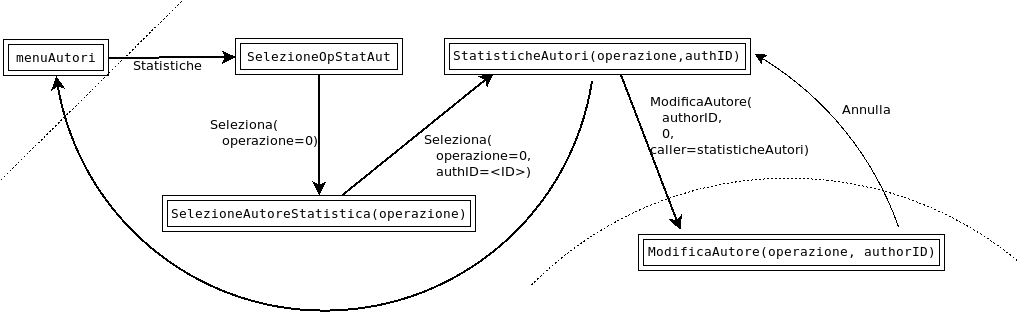
\includegraphics[width=\textwidth]{img/statAutori-0.png}\\[1cm]

\subsubsection{Collaborazioni effettuate}
\label{Collaborazioni}
\begin{itemize}
	\item \textbf{Procedure coinvolte}: SelezioneOpStatAut, SelezioneAutoreStatistica, StatisticheAutori
	\item \textbf{Obiettivo}: Visualizza le opere realizzate in collaborazione con altri autori presenti nella base di dati (anche nessuna)
	\item \textbf{Parametri}:
	\begin{enumerate}
		\item \textbf{operazione}: in number
		\item \textbf{authID}: in number
	\end{enumerate}
	\item \textbf{Risultato}: Stampa una pagina contenente tutte le opere realizzate dall'autore specificato ed un altro autore, raggruppandole per collaboratore
	\item \textbf{Errori}: nessuno
	\item \textbf{Usa}: Autori, Opere, AutoriOpere
	\item \textbf{Modifica}: nessuna
	\item \textbf{Precondizioni}:
	\begin{itemize}
		\item $\exists x \in Autori : x.IdAutore = AuthorID$
		\item $operazione  = 2$
	\end{itemize}
	\item \textbf{Postcondizioni}: nessuna
	\item \textbf{Note}: Poiché le opere sono raggruppate secondo il collaboratore
	è possibile che la stessa opera compaia più di una volta nella lista, sotto autori
	diversi
\end{itemize}
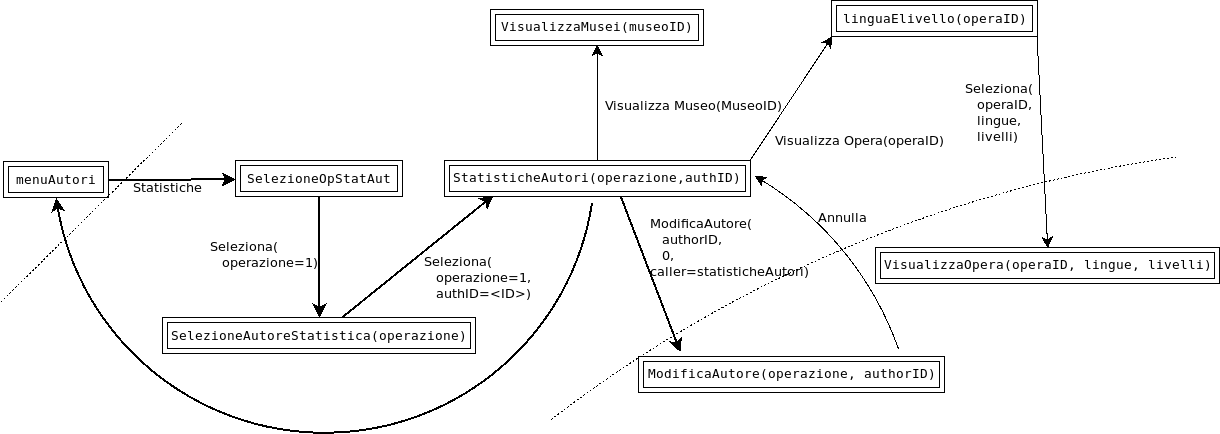
\includegraphics[width=\textwidth]{img/statAutori-1.png}\\[1cm]

\subsubsection{Opere dell’Autore presenti in un Museo scelto}
\begin{itemize}
	\item \textbf{Procedure coinvolte}: SelezioneOpStatAut, SelezioneAutoreStatistica, 
	StatisticheMuseoAutori
	\item \textbf{Obiettivo}: Visualizza le opere dell'autore specificato che sono esposte 
	nel museo scelto
	\item \textbf{Parametri}:
	\begin{enumerate}
		\item \textbf{operazione}: in number
		\item \textbf{authID}: in number
		\item \textbf{museoID}: in number
	\end{enumerate}
	\item \textbf{Risultato}: Stampa una pagina contenente tutte le opere realizzate dall'autore specificato che sono esposte all'interno del museo scelto
	\item \textbf{Errori}: nessuno
	\item \textbf{Usa}: Autori, Opere, AutoriOpere, Musei, SaleOpere, Stanze
	\item \textbf{Modifica}: nessuna
	\item \textbf{Precondizioni}:
	\begin{itemize}
		\item $\exists x \in Autori : x.IdAutore = AuthorID$
		\item $\exists y \in Musei : y.IdAutore = MuseoID$
		\item $operazione  = 3$
	\end{itemize}
	\item \textbf{Postcondizioni}: nessuna
\end{itemize}
%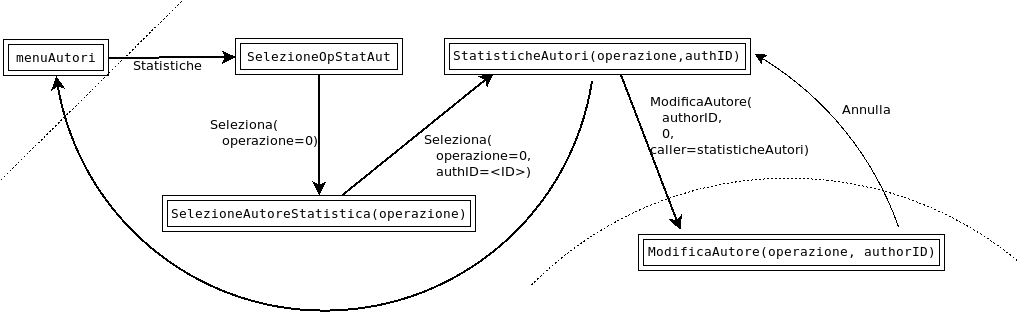
\includegraphics[width=\textwidth]{img/statAutori-0.png}\\[1cm]

\subsubsection{Autori in vita le cui Opere sono esposte in un Museo scelto}
\begin{itemize}
	\item \textbf{Procedure coinvolte}: SelezioneOpStatAut, SelezioneAutoreStatistica, 
	StatisticheMuseoAutori
	\item \textbf{Obiettivo}: Visualizza gli autori in vita (la cui data di morte è nulla)
	le cui opere sono esposte nel museo scelto
	\item \textbf{Parametri}:
	\begin{enumerate}
		\item \textbf{operazione}: in number
		\item \textbf{museoID}: in number
	\end{enumerate}
	\item \textbf{Risultato}: Stampa una pagina contenente tutti gli autori in vita
	 le cui opere sono esposte (potrebbero essere anche in prestito da un altro museo) 
	\item \textbf{Errori}: nessuno
	\item \textbf{Usa}: Autori, Opere, AutoriOpere, Musei, SaleOpere, Stanze
	\item \textbf{Modifica}: nessuna
	\item \textbf{Precondizioni}:
	\begin{itemize}
		\item $\exists y \in Musei : y.IdAutore = MuseoID$
		\item $operazione  = 4$
	\end{itemize}
	\item \textbf{Postcondizioni}: nessuna
	\item \textbf{Note}: Il parametro authID appare nell'URL nella pagina di 
	visualizzazione, ma soltanto con il valore di default: in realtà viene ignorato nella 
	logica dell'operazione
\end{itemize}

\subsubsection{Autori più prolifici (primi tre)}
\begin{itemize}
	\item \textbf{Procedure coinvolte}: SelezioneOpStatAut,SelezioneAutoreStatistica, classificaAutori
	\item \textbf{Obiettivo}: Visualizza i tre autori che hanno il maggior numero di opere
	all'interno della base di dati
	\item \textbf{Parametri}:
	\begin{enumerate}
		\item \textbf{operazione}: in number, in questo caso operazione=5
	\end{enumerate}
	\item \textbf{Risultato}: la lista dei tre autori che hanno realizzato più opere nella base di dati
	\item \textbf{Errori}: nessuno
	\item \textbf{Usa}: AutoriOpere, Autori
	\item \textbf{Modifica}: nessuno
	\item \textbf{Precondizioni}: nessuna
	\item \textbf{Postcondizioni}: nessuna
\end{itemize}

\clearpage

%%%%%%%%%%%%%%%%%%%%%%%%%%%%%%%%
% Operazioni sulle Descrizioni %
%%%%%%%%%%%%%%%%%%%%%%%%%%%%%%%%
\section{Operazioni sulle Descrizioni}

%%%%%%%%%%%%%%%%%%%%%%%%%%%%%%
%   Visualizza Descrizione   %
%%%%%%%%%%%%%%%%%%%%%%%%%%%%%%
\subsection{Visualizzazione}
\begin{itemize}
	\item \textbf{Operazione}: visualizzaDescrizione
	\item \textbf{Obiettivo}: Visualizza la Descrizione di un'Opera, dato il suo IdDescr
	\item \textbf{Parametri}:
	\begin{enumerate}
		\item \textbf{idSessione}: in (da definire)
		\item \textbf{DescrID}: in number(5)
	\end{enumerate}
	\item \textbf{Risultato}: Visualizza i dettagli della Descrizione richiesta, altrimenti restituisce errore
	\item \textbf{Errori}: 
	\begin{itemize}
		\item La descrizione richiesta non è presente nella base di dati
	\end{itemize}
	\item \textbf{Usa}: Descrizioni
	\item \textbf{Modifica}: Descrizioni
	\item \textbf{Precondizioni}:
	\begin{itemize}
		\item $\exists x \in Descrizioni : x.IdDescr = DescrID$
	\end{itemize}
	\item \textbf{Postcondizioni}: nessuna
\end{itemize}

%%%%%%%%%%%%%%%%%%%%%%%%%%%%%%
%   Inserisci Descrizione   %
%%%%%%%%%%%%%%%%%%%%%%%%%%%%%%
\subsection{Inserimento}
\begin{itemize}
	\item \textbf{Operazione}: inserisciDescrizione
	\item \textbf{Obiettivo}: Inserisce una nuova descrizione, associandola ad un'Opera
	\item \textbf{Parametri}:
	\begin{enumerate}
		\item \textbf{idSessione}: in (da definire)
		\item \textbf{lingua}: in varchar2(25)
		\item \textbf{livello}: in varchar2(25)
		\item \textbf{testodescr}: in CLOB
		\item \textbf{OperaID}: in number(5)
	\end{enumerate}
	\item \textbf{Risultato}: Inserisce la descrizione dell'Opera, restituisce errore se l'Opera non è presente nel database
	\item \textbf{Errori}: 
	\begin{itemize}
		\item L'Opera a cui associare la descrizione non è presente nella base di dati
	\end{itemize}
	\item \textbf{Usa}: Descrizioni, Opere
	\item \textbf{Modifica}: Descrizioni
	\item \textbf{Precondizioni}:
	\begin{itemize}
		\item $\exists x \in Opere : x.IdOpera = OperaID$
	\end{itemize}
	\item \textbf{Postcondizioni}:
	\begin{itemize}
		\item $\exists x \in Descrizioni : x.Opera = OperaID \land x.Lingua = lingua \land x.Livello = livello \land x.Testo = testodescr$
	\end{itemize}
\end{itemize}

%%%%%%%%%%%%%%%%%%%%%%%%%%%%%%
%    Modifica Descrizione    %
%%%%%%%%%%%%%%%%%%%%%%%%%%%%%%
\subsection{Modifica}
\begin{itemize}
	\item \textbf{Operazione}: ModificaDescrizione
	\item \textbf{Obiettivo}: Modifica la descrizione di un'opera (è possibile modificare anche l'opera a cui una descrizione è associata)
	\item \textbf{Parametri}:
	\begin{enumerate}
		\item \textbf{idSessione}: in (da definire)
		\item \textbf{descrID}: in number(5)
		\item \textbf{newlang}: in varchar2(25) default null
		\item \textbf{newlevel}: in varchar2(25) default null
		\item \textbf{newtext}: in CLOB default null
		\item \textbf{newOpera}: in number(5) default null
	\end{enumerate}
	\item \textbf{Risultato}: Modifica gli attributi della descrizione individuata da descrID, oppure ritorna un errore
	\item \textbf{Errori}: 
	\begin{itemize}
		\item La descrizione da modificare non è presente nella base di dati
		\item La nuova Opera da associare alla descrizione non è presente nella base di dati
	\end{itemize}
	\item \textbf{Usa}: Opere, Descrizioni
	\item \textbf{Modifica}: Descrizioni
	\item \textbf{Precondizioni}:
	\begin{itemize}
		\item $\exists x \in Descrizioni : x.IdDescr = descrID$
		\item $\exists x \in Opere : x.IdOpera = newOpera$
	\end{itemize}
	\item \textbf{Postcondizioni}:
	\begin{align*} (\exists x \in Descrizioni.
		& (newlang \ne null \Rightarrow x.Lingua = newlang) \\
		& \land (newlevel \ne null \Rightarrow x.Livello = newlevel) \\
		& \land (newtext \ne null \Rightarrow x.Testo = newtext) \\
		& \land (newOpera \ne null \Rightarrow x.Opera = newOpera))
	\end{align*}
\end{itemize}

%%%%%%%%%%%%%%%%%%%%%%%%%%%%%%
%   Rimozione Descrizione    %
%%%%%%%%%%%%%%%%%%%%%%%%%%%%%%
\subsection{Rimozione}
\begin{itemize}
	\item \textbf{Operazione}: rimuoviDesrizione
	\item \textbf{Obiettivo}: Rimuove una descrizione, se presente
	\item \textbf{Parametri}:
	\begin{enumerate}
		\item \textbf{idSessione}: in (da definire)
		\item \textbf{descrID}: in number(5)
	\end{enumerate}
	\item \textbf{Risultato}: Rimuove la descrizione dell'Opera, restituendo errore se la descrizione non è presente nel database
	\item \textbf{Errori}: 
	\begin{itemize}
		\item La Descrizione identificata da descrID non è presente nella base di dati
	\end{itemize}
	\item \textbf{Usa}: Descrizioni
	\item \textbf{Modifica}: Descrizioni
	\item \textbf{Precondizioni}:
	\begin{itemize}
		\item $\exists x \in Descrizioni : x.IdDescr = descrID$
		\item $|Descrizioni| = n$
	\end{itemize}
	\item \textbf{Postcondizioni}:
	\begin{itemize}
		\item $\nexists x \in Descrizioni : x.IdDescr = descrID$
		\item $|Descrizioni| = n - 1$
	\end{itemize}
\end{itemize}

%%%%%%%%%%%%%%%%%%%%%%%%%%%%%%
%   Statistiche e monitoraggio Descrizioni    %
%%%%%%%%%%%%%%%%%%%%%%%%%%%%%%
\subsection{Statistiche e monitoraggio}
\begin{itemize}
	\item \textbf{Operazione}: StatisticheDescrizioni
	\item \textbf{Obiettivo}: Visualizza le statistiche delle descrizioni
	\item \textbf{Parametri}: nessuno
	\item \textbf{Risultato}: Visualizza i titoli e le statistiche disponibili riguardanti le descrizioni
	\item \textbf{Errori}: nessuno
	\item \textbf{Usa}: Descrizioni
	\item \textbf{Modifica}: nessuna
	\item \textbf{Precondizioni}: nessuna
	\item \textbf{Postcondizioni}: nessuna
	\item \textbf{Note}: Vengono sempre eseguite tutte le operazioni di statistica
\end{itemize}

%%%%%%%%%%%%%%%%%%%%%%%%%%%%%%
%   Livello descrizione più presente    %
%%%%%%%%%%%%%%%%%%%%%%%%%%%%%%
\subsubsection{Livello descrizione più presente}
\begin{itemize}
	\item \textbf{Obiettivo}: Visualizza il livello più presente nelle descrizioni e il numero di descrizioni che lo possiedono
	\item \textbf{Parametri}: nessuno
	\item \textbf{Risultato}: Visualizza il livello di descrizione più presente e il numero di opere che lo possiedono (in caso di più livelli con il massimo valore, vengono tutti mostrati) oppure non mostra niente
	\item \textbf{Errori}: nessuno
	\item \textbf{Usa}: Descrizioni
	\item \textbf{Modifica}: nessuna
	\item \textbf{Precondizioni}: nessuna
	\item \textbf{Postcondizioni}: nessuna
\end{itemize}

%%%%%%%%%%%%%%%%%%%%%%%%%%%%%%
%   Lingua descrizione più presente    %
%%%%%%%%%%%%%%%%%%%%%%%%%%%%%%
\subsubsection{Lingua più presente}
\begin{itemize}
	\item \textbf{Obiettivo}: Visualizza la lingua più presente nelle descrizioni e il numero di descrizioni che la possiedono
	\item \textbf{Parametri}: nessuno
	\item \textbf{Risultato}: Visualizza la lingu di descrizione più presente e il numero di opere che la possiedono (in caso di più lingue con il massimo valore, vengono tutti mostrate) oppure non mostra niente
	\item \textbf{Errori}: nessuno
	\item \textbf{Usa}: Descrizioni
	\item \textbf{Modifica}: nessuna
	\item \textbf{Precondizioni}: nessuna
	\item \textbf{Postcondizioni}: nessuna
\end{itemize}


\end{document}
